\chapter{Planejamento das Avaliações}

\section{Divisão das metas nas iterações}
\begin{figure}[h!]
  \centering
    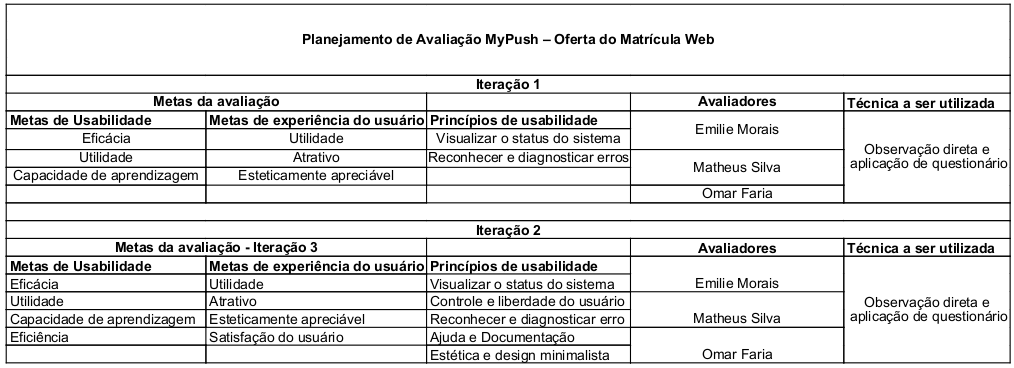
\includegraphics[keepaspectratio=true, scale=0.5]{figuras/planejamentoavaliacoes.png}
  \caption{Planejamento das avaliações}
\end{figure}

% \begin{figure}[h!]
%   \centering
%     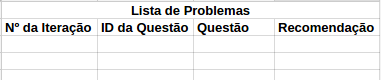
\includegraphics[keepaspectratio=true, scale=0.7]{figuras/listaproblemas.png}
%   \caption{Lista de problemas a ser preenchida nas avaliações}
% \end{figure}
% 

\section{Resultados qualitativos}

\subsection{Método de investigação}
Através de uma rápida entrevista com o usuário serão obtidas algumas informações além do questionário.

\subsection{Problemas encontrados nas avaliações}

Se o usuário durante ou depois da avaliação relatar algum problema, o mesmo deve ser registrado na tabela abaixo.
\begin{table*}[!h]
\caption{Lista de problemas a ser preenchida nas avaliações. Fonte: \cite{preece} adaptado}
\label{Rotulo}
  \begin{tabular}{p{0.18\linewidth}p{0.18\linewidth}p{0.30\linewidth}p{0.30\linewidth}}
  \hline
    Nº da Iteração & ID da Questão & Questão & Recomendação\\
 \hline
  \end{tabular}
\end{table*}

\section{Resultados quantitativos}

  \subsection{Método de investigação}
  Cada questão dos questionário será avaliada de 0 a 5 e assim serão obtidos resultados numéricos
  em relação a cada meta a ser avaliada.

  
  \subsection{Método de inspeção}
  Esse método será aplicado na versão \textit{Desktop} do protótipo de modo a avaliar a acessibilidade da página.
  
  \subsection{Método de observação}
  Serão obtidos valores numéricos para algumas metas utilizando-se de métricas de qualidade obtidas na
  norma \citeonline{iso}.
  
\vfill
\pagebreak
\subsubsection{Métricas a serem utilizadas nas avaliações}
\begin{figure}[!h]
  \centering
    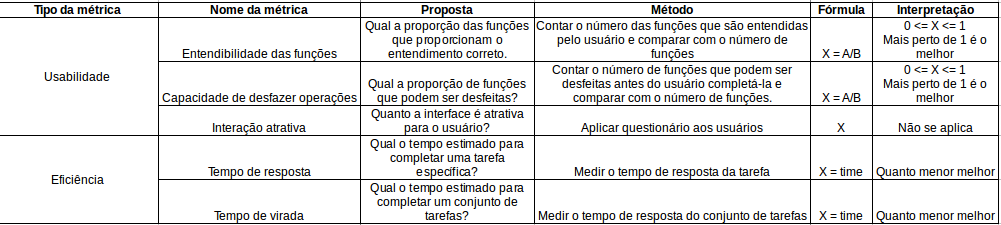
\includegraphics[keepaspectratio=true, scale=0.6, angle=-90]{figuras/qualidade.png}
  \caption{Métricas de Qualidade. Fonte: \cite{iso}}
\end{figure}

\pagebreak

\section{Iteração 1}

\begin{figure}[h!]
  \centering
    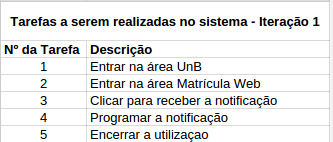
\includegraphics[keepaspectratio=true, scale=0.7]{figuras/tarefas1.png}
  \caption{Lista de Tarefas para os usuários na Iteração 1}
\end{figure}

\begin{table*}[!h]
\caption{Lista de problemas. Fonte: \cite{preece} adaptado}
\label{Rotulo}
  \begin{tabular}{p{0.18\linewidth}p{0.18\linewidth}p{0.30\linewidth}p{0.30\linewidth}}
  \hline
    Nº da Iteração & ID da Questão & Questão & Recomendação\\
 \hline
  \end{tabular}
\end{table*}